\documentclass{beamer}

% ==========================================
% THEME AND PACKAGES
% ==========================================

\usetheme{Boadilla}

\usepackage{tikz}
\usepackage{graphicx}
\usepackage{xcolor}

\usefonttheme{serif}
\usecolortheme{default}

% ==========================================
% WHITE + BURGUNDY + ROSE GOLD THEME
% ==========================================

\definecolor{whitebg}{RGB}{255,255,255}
\definecolor{burgundy}{RGB}{66,28,43}
\definecolor{darkwine}{RGB}{48,19,31}
\definecolor{winepanel}{RGB}{104,64,75}
\definecolor{rosegold}{RGB}{197,139,131}
\definecolor{ivory}{RGB}{246,239,234}
\definecolor{blush}{RGB}{248,237,235}

% ==========================================
% BACKGROUND AND TEXT
% ==========================================

\setbeamercolor{normal text}{
    fg=burgundy,
    bg=whitebg
}

\setbeamercolor{background canvas}{
    bg=whitebg
}

\setbeamercolor{structure}{
    fg=burgundy
}

% ==========================================
% TITLE AND HEADINGS
% ==========================================

\setbeamercolor{title}{
    fg=ivory,
    bg=darkwine
}

\setbeamercolor{titlelike}{
    fg=burgundy,
    bg=whitebg
}

\setbeamercolor{frametitle}{
    fg=ivory,
    bg=burgundy
}

\setbeamercolor{subtitle}{
    fg=rosegold
}

% ==========================================
% AUTHOR AND DATE
% ==========================================

\setbeamercolor{author}{
    fg=burgundy
}

\setbeamercolor{date}{
    fg=burgundy
}

% ==========================================
% NORMAL BLOCKS
% ==========================================

\setbeamercolor{block title}{
    fg=ivory,
    bg=burgundy
}

\setbeamercolor{block body}{
    fg=burgundy,
    bg=blush
}

% ==========================================
% ALERT BLOCKS
% ==========================================

\setbeamercolor{alertblock title}{
    fg=white,
    bg=rosegold
}

\setbeamercolor{alertblock body}{
    fg=burgundy,
    bg=blush
}

% ==========================================
% EXAMPLE BLOCKS
% ==========================================

\setbeamercolor{exampleblock title}{
    fg=ivory,
    bg=darkwine
}

\setbeamercolor{exampleblock body}{
    fg=burgundy,
    bg=blush
}

% ==========================================
% HEADER AND FOOTER
% ==========================================

\setbeamercolor{palette primary}{
    fg=ivory,
    bg=darkwine
}

\setbeamercolor{palette secondary}{
    fg=white,
    bg=rosegold
}

\setbeamercolor{palette tertiary}{
    fg=ivory,
    bg=burgundy
}

\setbeamercolor{palette quaternary}{
    fg=ivory,
    bg=darkwine
}

\setbeamercolor{author in head/foot}{
    fg=ivory,
    bg=darkwine
}

\setbeamercolor{date in head/foot}{
    fg=white,
    bg=rosegold
}

% ==========================================
% TABLE OF CONTENTS
% ==========================================

\setbeamercolor{section in toc}{
    fg=burgundy
}

\setbeamercolor{subsection in toc}{
    fg=rosegold
}

% ==========================================
% BULLET POINTS
% ==========================================

\setbeamercolor{itemize item}{
    fg=rosegold
}

\setbeamercolor{itemize subitem}{
    fg=burgundy
}

\setbeamercolor{enumerate item}{
    fg=rosegold
}

% ==========================================
% REMOVE NAVIGATION SYMBOLS
% ==========================================

\setbeamertemplate{navigation symbols}{}

% ==========================================
% PRESENTATION DETAILS
% ==========================================

\title[Campus Course Management]
{\textbf{Campus Course Management System}}

\author[]{
\textbf{Project Team}\\
\vspace{0.2cm}
Shalini -CS25BT020\\
Premi -CS25BT022\\
Akshitha -CS25BT030\\
Ridhima -CS25BT033\\
Tejaswini -CS25BT043\\
\vspace{0.2cm}
\textbf{Instructor:Dr. Suman Dutta}\\
Computer Science and Engineering\\
Indian Institute of Technology, Dharwad
}

\date{16 November 2026}

% ==========================================
% DOCUMENT START
% ==========================================

\begin{document}

% ==========================================
% SLIDE 1: TITLE
% ==========================================

\begin{frame}[plain]

\titlepage

\end{frame}

% ==========================================
% SLIDE 2: INTRODUCTION AND PROBLEM STATEMENT
% ==========================================

\begin{frame}{Introduction and Problem Statement}

\begin{block}{Project Overview}

The Campus Course Management System is a web-based
application designed to simplify academic activities
within a college.

\end{block}

\textbf{\color{burgundy}Our system provides facilities for:}

\begin{enumerate}
    \item Students
    \item Faculty Members
    \item Administrators (accessed through backend server)
\end{enumerate}

\begin{block}{Problem Statement}

Manage students, faculty, courses, enrollment, assignments and grades. Provide search, update, reporting and role-based operations through a Java application with persistent storage.

\end{block}



\end{frame}

% ==========================================
% SLIDE 3: TECHNOLOGIES AND ARCHITECTURE
% ==========================================

\begin{frame}{Technologies and System Architecture}

\begin{block}{Technologies Used}

\begin{itemize}

    \item \textbf{Backend:} Python, Django, Django REST Framework, JWT authentication

    \item \textbf{Frontend:} React 19, React Router, Vite, JavaScript, CSS

    \item \textbf{Database:} SQLite (managed through the Django ORM)

    \item \textbf{Tools:} Git and GitHub

\end{itemize}

\end{block}

\textbf{\color{burgundy}System Architecture}

\vspace{0.3cm}

\begin{center}

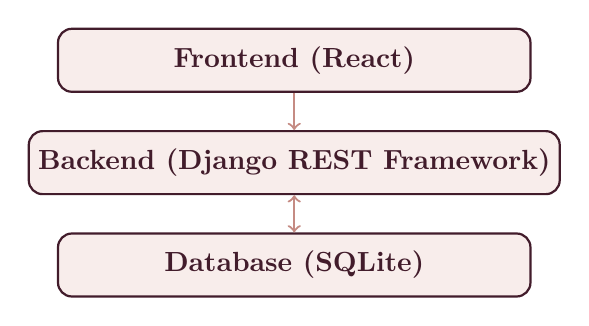
\begin{tikzpicture}

    \node[
        draw=burgundy,
        fill=blush,
        text=burgundy,
        rounded corners=5pt,
        minimum width=6cm,
        minimum height=0.8cm,
        thick
    ]
    (a) at (0,2) {\textbf{Frontend (React)}};

    \node[
        draw=burgundy,
        fill=blush,
        text=burgundy,
        rounded corners=5pt,
        minimum width=6cm,
        minimum height=0.8cm,
        thick
    ]
    (b) at (0,0.7) {\textbf{Backend (Django REST Framework)}};

    \node[
        draw=burgundy,
        fill=blush,
        text=burgundy,
        rounded corners=5pt,
        minimum width=6cm,
        minimum height=0.8cm,
        thick
    ]
    (c) at (0,-0.6) {\textbf{Database (SQLite)}};

    \draw[->,thick,rosegold] (a) -- (b);

    \draw[<->,thick,rosegold] (b) -- (c);

\end{tikzpicture}

\end{center}

\end{frame}

% ==========================================
% SLIDE 4: PROJECT IMPLEMENTATION
% ==========================================

\begin{frame}{Project Implementation}

\begin{block}{Backend Development}

The backend handles the main operations of our system.

\begin{itemize}

    \item User Authentication and Role Management
    \item Course Management
    \item Assignment Management
    \item Assignment Submission
    \item API Development

\end{itemize}



\end{block}

\begin{block}{Frontend Development}

The frontend provides an interactive interface
for different users.
Login Page,
     Student Dashboard,
     Faculty Dashboard,
     Admin Dashboard,
 Course and Assignment Pages


\end{block}

\end{frame}

% ==========================================
% SLIDE 5: DATABASE AND TEAM CONTRIBUTIONS
% ==========================================

\begin{frame}{Database Design and Team Contributions}

\begin{block}{Database Design}

We use SQLite to store and manage application information.

\begin{itemize}

    \item Users
    \item Students
    \item Faculty
    \item Courses
    \item Assignments
    \item Submissions

\end{itemize}

\end{block}




\end{frame}

% ==========================================
% SLIDE 6: DEMONSTRATION AND CONCLUSION
% ==========================================

\begin{frame}{Project Demonstration and Conclusion}

\begin{center}

\textbf{\color{burgundy}Login Page}

\vspace{0.2cm}

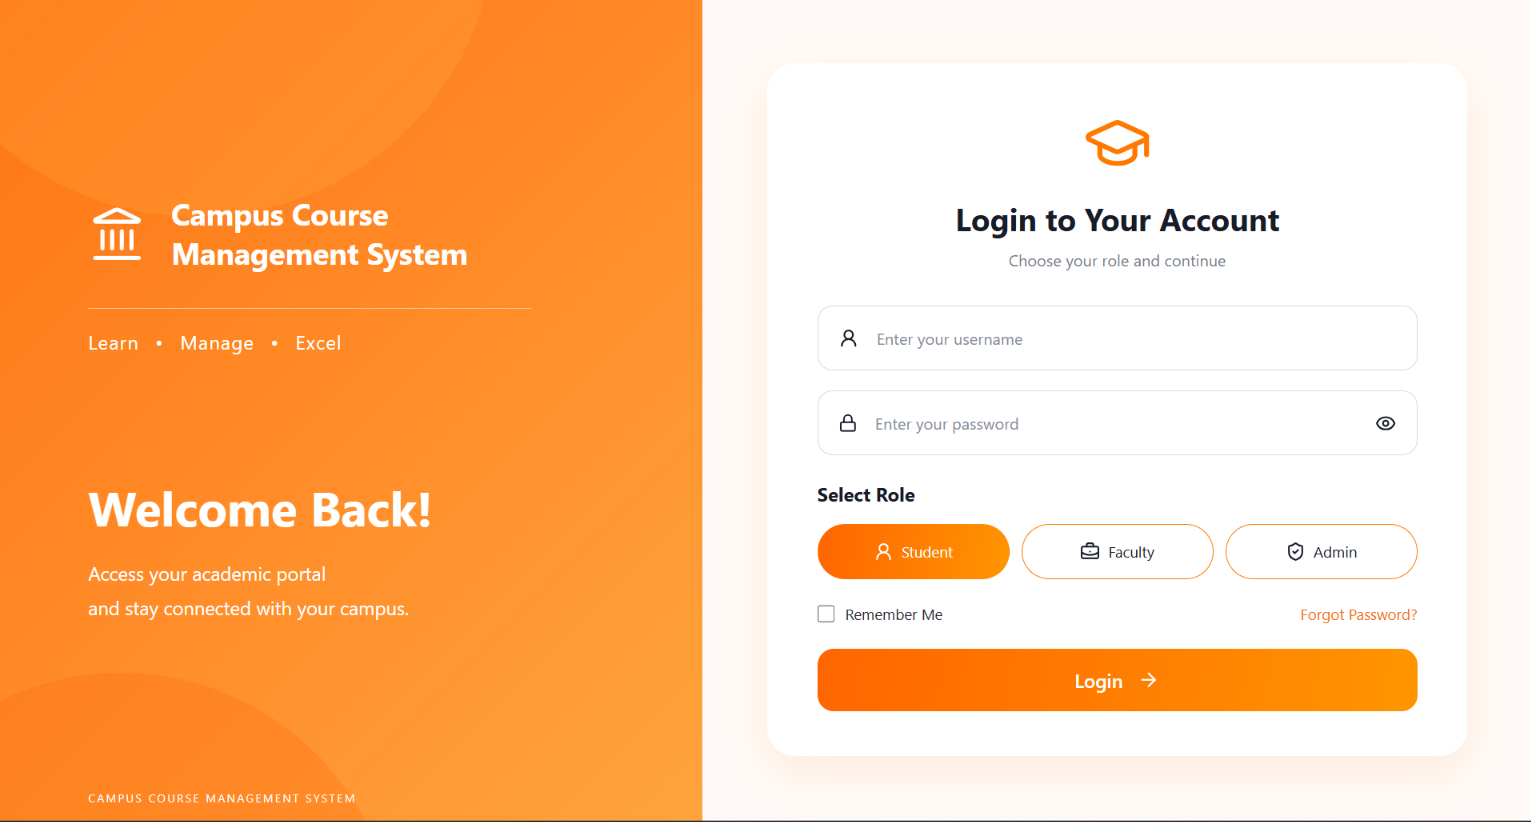
\includegraphics[width=0.9\textwidth]{login.png}

\end{center}



\end{frame}

% ==========================================
% SLIDE 7: THANK YOU
% ==========================================

\begin{frame}[plain]

\begin{center}

\vspace{0.5cm}


\includegraphics[width=0.73\textwidth]{page.png}

\vspace{0.4cm}

{\Huge\textbf{\color{burgundy}Thank You!}}

\vspace{0.3cm}

{\large\color{rosegold}Questions?}

\end{center}

\end{frame}

% ==========================================
% DOCUMENT END
% ==========================================

\end{document}